% Results of the first trained model: unconditioned factored attention, H = 128.
% Numbers from evaluations/fa_unconditional_H128/{metrics,tree_comparison,mode_mixing}.json

\section{Results: the unconditioned model with $H=128$}\label{sec:res_uncond}

\subsection{What was trained}
The unconditioned model of \S\ref{sec:fa} was trained on all 144{,}000 training sequences (18 clades, no tags).
At your request it used $\bm{H=128}$ heads instead of the 256 of the plan, i.e.\ 543{,}920 parameters
(run \texttt{fa\_unconditional\_H128}). Note that 128 is below the $\approx179$ heads that the rank argument
of \S\ref{sec:rank} requires for an exact representation of our couplings. Everything else is as in
\S\ref{sec:plan}: pseudo-likelihood with $\lambda_h=\lambda_J=10^{-5}$, Adam ($5\times10^{-3}$), batch 512,
60 epochs. Training took 98\,s on the RTX~2060.

\begin{figure}[H]
\centering
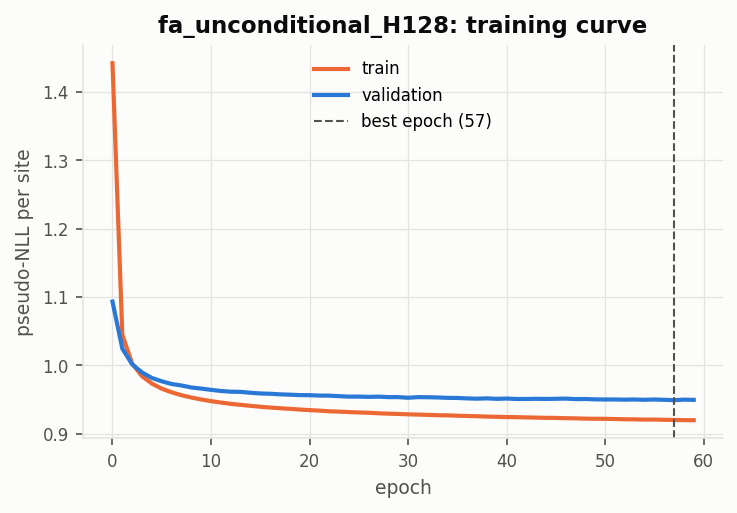
\includegraphics[width=0.55\linewidth]{models/fa_unconditional_H128/training_curve.png}
\caption{Training curve. Best validation pseudo-NLL per site: $0.949$ (epoch 57 of 60). It was still
decreasing slowly at the 60-epoch cap. The train/validation gap is small ($0.920$ vs $0.949$), so there is
little over-fitting.}
\end{figure}

For comparison (\S\ref{sec:plan}): an independent-site model scores 2.11, and the true clade models 0.80.
The unconditioned model reaches $0.95$. That is far better than independent sites, and it cannot reach
0.80, because a single Potts model cannot represent the mixture of 18 clade models.

Evaluation protocol (\S\ref{sec:evalprotocol}): 18{,}000 sequences Gibbs-sampled from the learned $(h,J)$
(200 sweeps, one sequence per chain), compared with the 18{,}000 held-out test sequences. The
\emph{oracle} is 18{,}000 fresh samples of the true clade models (1000 per clade), the best achievable score.

\subsection{Site frequencies and correlations}
\begin{center}\small
\begin{tabular}{lccccc}
\toprule
compared with the test set & $r_f$ & $r_C$ & slope $C$ & identity gen--gen & copies\\
\midrule
oracle (fresh true samples) & 1.000 & 0.994 & 0.99 & 0.197 & 0\%\\
\textbf{generated} & \textbf{0.940} & \textbf{0.895} & \textbf{0.70} & \textbf{0.260} & 0\%\\
generated, rebalanced to equal family shares$^\ast$ & 0.992 & 0.949 & 0.79 & 0.209 & 0\%\\
\bottomrule
\end{tabular}\\[2pt]
{\footnotesize $^\ast$ 2101 generated sequences from each family (see \S\ref{sec:res_props}); identity of the test set itself: 0.198.}
\end{center}

\begin{figure}[H]
\centering
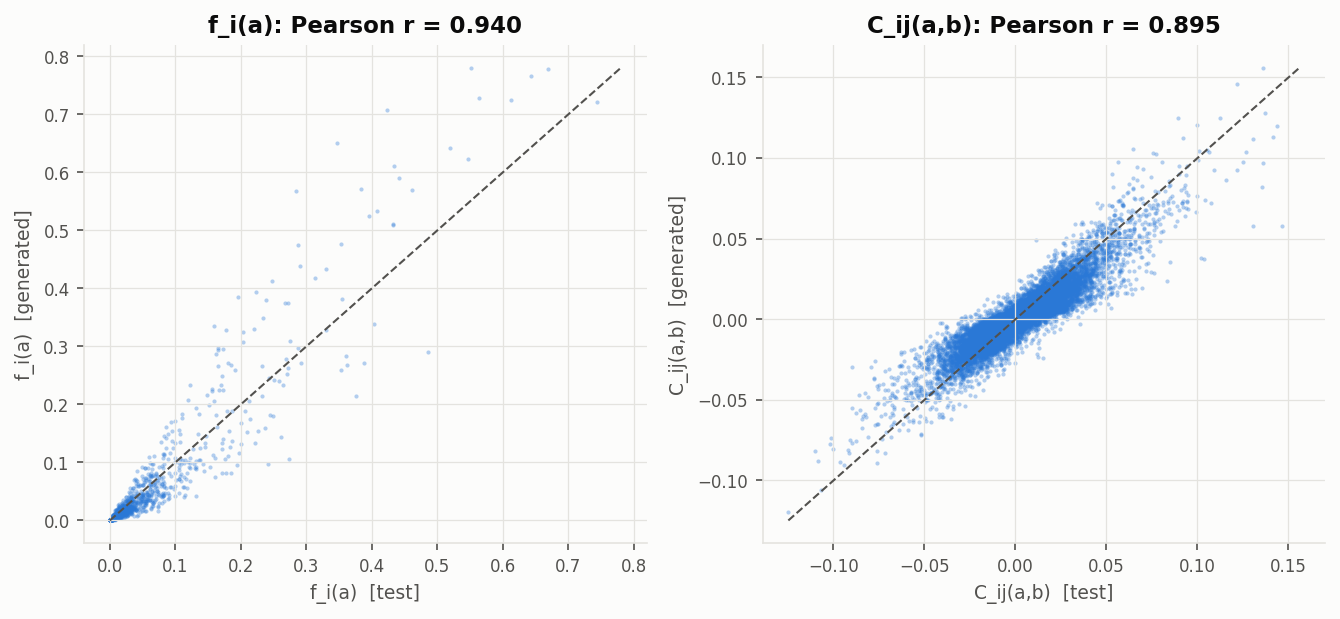
\includegraphics[width=0.49\linewidth]{models/fa_unconditional_H128/freq_corr_generated_vs_test.png}\hfill
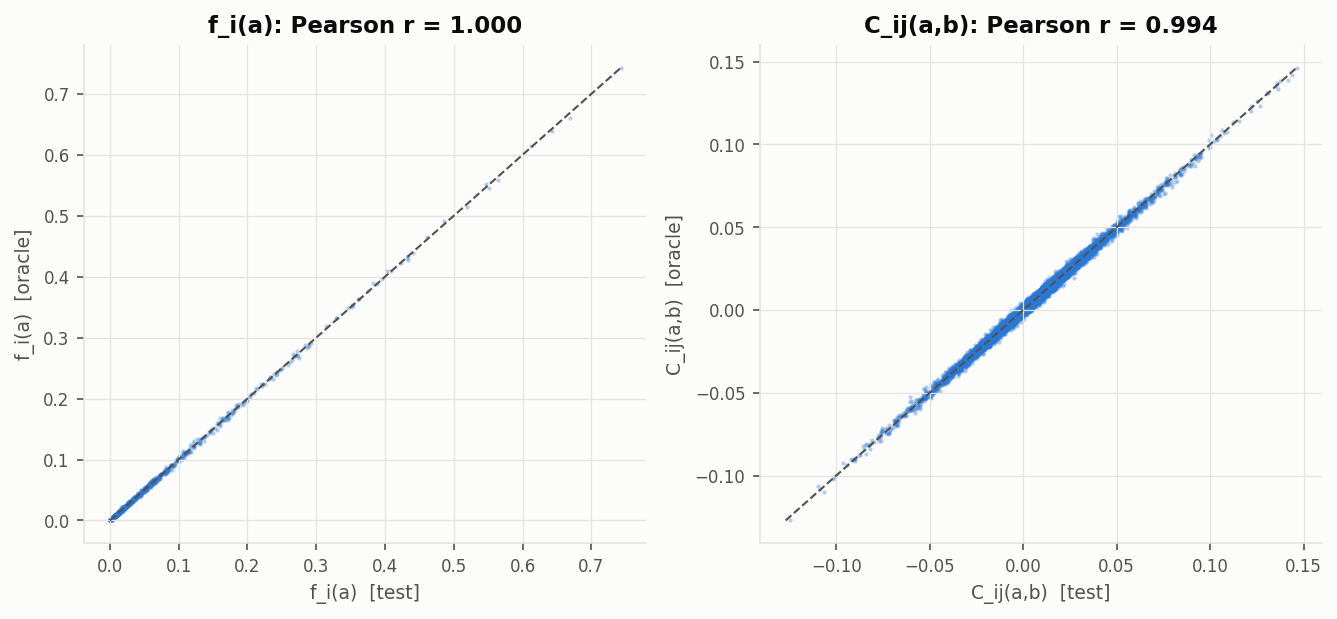
\includegraphics[width=0.49\linewidth]{models/fa_unconditional_H128/freq_corr_oracle_vs_test.png}
\caption{Site frequencies $f_i(a)$ and connected correlations $C_{ij}(a,b)$ of the generated sequences
(left pair) and of the oracle (right pair) against the test sequences. Points on the dashed line are
reproduced exactly.}
\end{figure}

\begin{figure}[H]
\centering
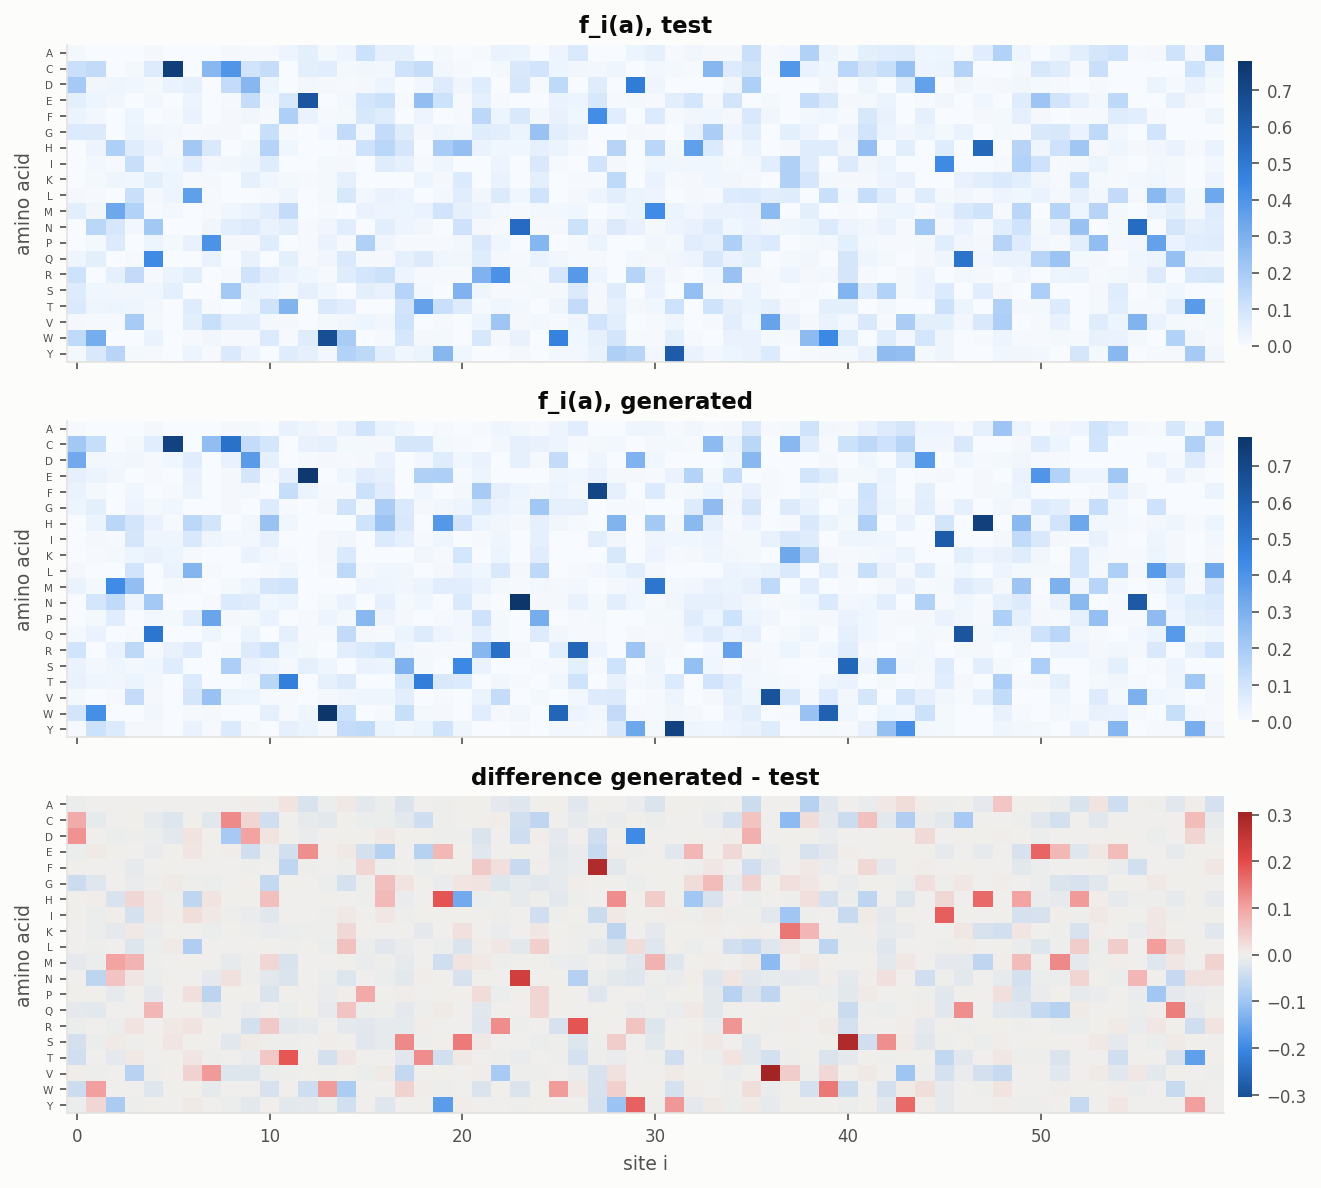
\includegraphics[width=0.78\linewidth]{models/fa_unconditional_H128/site_frequencies_test_vs_generated.png}
\caption{Site frequencies of the test set, of the generated set, and their difference (red: too frequent
in the generated sequences, blue: too rare). The errors are concentrated on a few residues at a few sites.
These are the residues that distinguish the families (next subsection).}
\end{figure}

\begin{figure}[H]
\centering
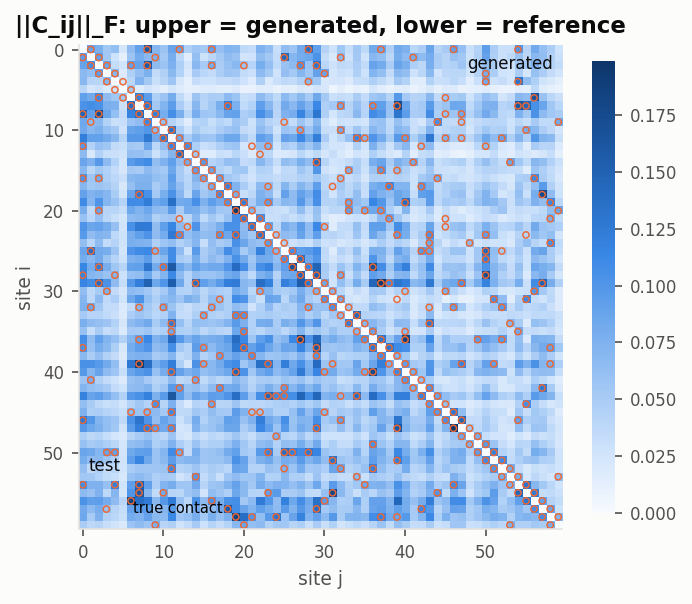
\includegraphics[width=0.5\linewidth]{models/fa_unconditional_H128/correlation_strength_test_vs_generated.png}
\caption{Strength of the correlation between every pair of sites, $\|C_{ij}\|_F$. Lower triangle: test set;
upper triangle: generated; circles: true contacts. In the \emph{pooled} data almost all pairs are correlated,
not only contacts: sites whose preferred residue differs between families become correlated through the
family identity (the mixture effect of \S\ref{sec:cond}). The generated set reproduces this background and the
strongest contact correlations.}
\end{figure}

\subsection{Family proportions: the main failure}\label{sec:res_props}
Each generated sequence is assigned to the family whose test centroid is nearest on the reference PCA (all 10
components). Sequences farther from every centroid than 99\% of the test sequences are from their own
centroid count as ``between families'' (\texttt{family\_assignment}).
\begin{center}\small
\begin{tabular}{lcccc}
\toprule
 & F0 & F1 & F2 & between\\
\midrule
test & 33.0\% & 32.7\% & 33.3\% & 1.0\%\\
oracle & 33.1\% & 32.7\% & 33.3\% & 0.9\%\\
\textbf{generated} & \textbf{21.7\%} & \textbf{11.6\%} & \textbf{66.4\%} & 0.3\%\\
\bottomrule
\end{tabular}
\end{center}

\begin{figure}[H]
\centering
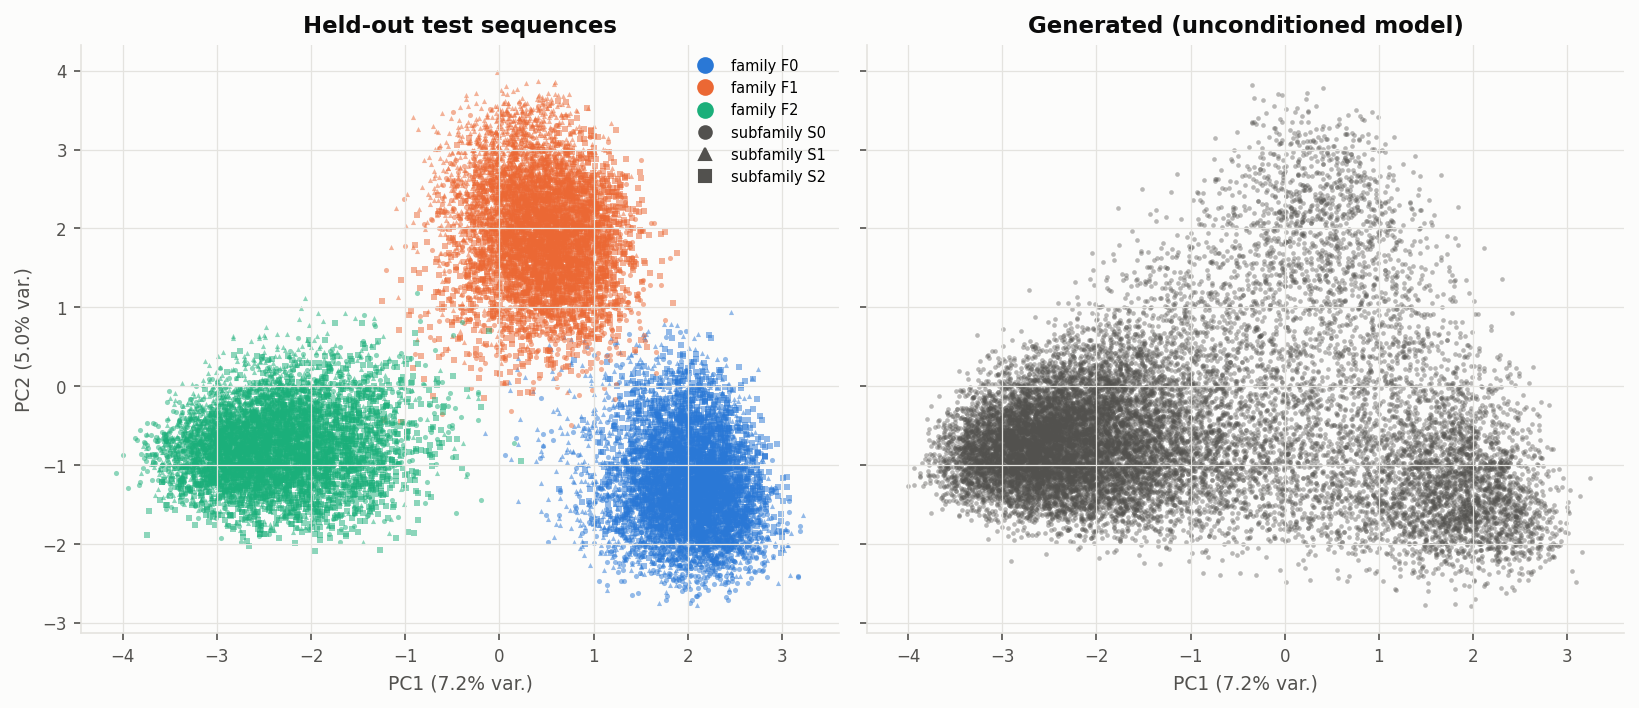
\includegraphics[width=0.85\linewidth]{models/fa_unconditional_H128/pca_generated_vs_test.png}
\caption{Test sequences (left, coloured by family) and generated sequences (right) on the reference PCA
axes of Part~I. The generated sequences occupy all three family regions, with the wrong weights: F2
(bottom left) is over-populated and F1 (top) under-populated.}
\end{figure}

\paragraph{Is it the model or the sampler?} With three well-separated families, a Gibbs chain could get
trapped in whichever family it falls into first. The proportions would then reflect the starting
points, not the learned distribution. We tested this (\texttt{s08\_mode\_mixing.py}): 600 chains were
started from random sequences, and 600 from the test sequences of each family. We then tracked where the
chains are after 100--500 sweeps.
\begin{figure}[H]
\centering
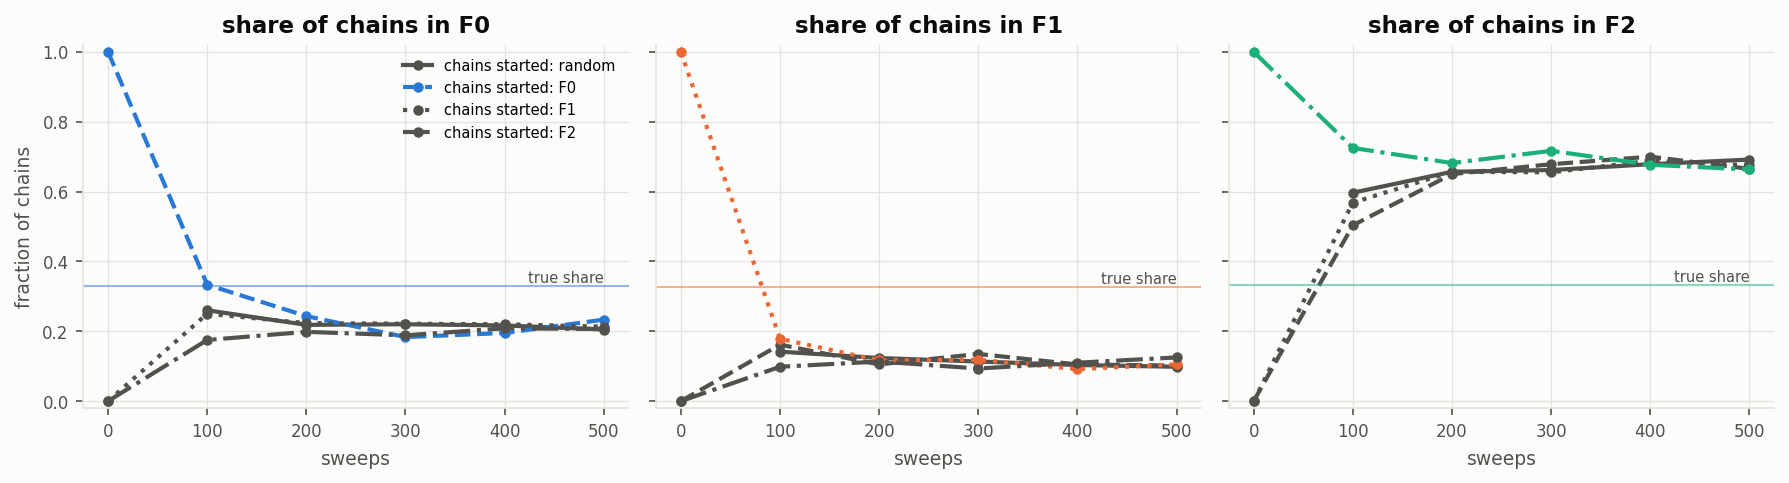
\includegraphics[width=\linewidth]{models/fa_unconditional_H128/mode_mixing.png}
\caption{Share of chains in each family vs sweeps, for chains started at random or inside F0, F1 or F2.
Chains started inside F0 or F1 leave it within 100--200 sweeps. All four starts converge to the same
$\approx20/11/68\%$ split. Horizontal lines: the true share $1/3$.}
\end{figure}
All starts converge to the same proportions, so \textbf{the sampler mixes between families and the
$20/11/68$ split is a property of the learned distribution itself.} Why would pseudo-likelihood learn wrong
family weights? The PL \eqref{eq:pl} only involves the conditionals $P(s_i\mid\s_{-i})$, which never compare
two \emph{different} regions of sequence space. The relative weight of two families is the ratio of the
total Boltzmann weight in each region, a global quantity set by $Z$, which PL never sees. As long as each
family's sequences are predicted well site by site, PL is nearly blind to how much weight each family
receives. This is a known weakness of PLM on multimodal data. The conditioned model avoids it by
construction, since the tag chooses the family.

\paragraph{Is it an energy effect? (``the sampler minimises the energy'')} Figure~\ref{fig:energytraces} shows that the clades of
F2 have the lowest mean energy, and F2 is the over-generated family, so it is natural to suspect that
sampling favours low energy. The link is real, but the mechanism is different. Two facts first:
\begin{itemize}[nosep]
\item Gibbs sampling does \emph{not} minimise the energy. It draws $\s$ with probability $e^{-E(\s)}/Z$
(validated against exact enumeration, \S\ref{sec:gibbstests}). High-energy sequences are rarer, not
excluded.
\item Figure~\ref{fig:energytraces} compares each clade under \emph{its own} model, and the clades were sampled
\emph{separately}. There the families never compete, which is why the oracle has exactly 1/3 in each.
\end{itemize}
In the learned (single) model, however, the three families do compete. The weight of family $F$ is the sum of
the Boltzmann weights of all sequences in its region:
\begin{equation}\label{eq:freeenergy}
P(F)=\frac1Z\sum_{\s\in F}e^{-E(\s)}=\frac1Z\,e^{-(\langle E\rangle_F-S_F)}
\quad\Longrightarrow\quad
\ln\frac{P(F)}{P(F')}=\underbrace{-\big(\langle E\rangle_F-\langle E\rangle_{F'}\big)}_{\text{energy term}}
+\underbrace{\big(S_F-S_{F'}\big)}_{\text{entropy term}}
\end{equation}
where $\langle E\rangle_F$ is the mean energy of the model restricted to region $F$ and $S_F$ its entropy,
i.e.\ the logarithm of the effective number of sequences in $F$. (The second equality defines $S_F$: write
$\sum_{\s\in F}e^{-E}=e^{-\langle E\rangle_F}\sum_{\s\in F}e^{-(E-\langle E\rangle_F)}$ and call the log of the
last sum $S_F$. It is exactly the Gibbs entropy of the restricted distribution.) A family can therefore win
either by having low energies or by having many sequences. We measured the energy term with 2400 samples of the
learned model and obtained the entropy term as the remainder (\texttt{s08\_mode\_mixing.py}):
\begin{center}\small
\begin{tabular}{lccccc}
\toprule
family & $\langle E\rangle_F$ & energy term & entropy term & $\ln\frac{P(F)}{P(\text{F2})}$ & site entropy\\
 & (learned model) & vs F2 & vs F2 & & (test seqs)\\
\midrule
F0 & $-176.1$ & $-10.7$ & $+9.6$ & $-1.12$ & 1.87\\
F1 & $-173.1$ & $-13.7$ & $+12.1$ & $-1.60$ & 1.94\\
F2 & $-186.8$ & 0 & 0 & 0 & 1.57\\
\bottomrule
\end{tabular}
\end{center}
F2 is the most conserved family: lowest site entropy, highest identity (0.36). Hence, in the learned model,
its sequences have $\approx11$--14 units lower energy, but its region also holds far fewer sequences. The two
effects almost cancel: an energy advantage worth a factor $e^{11}\approx60{,}000$ is reduced to a factor
$\approx3$--5 by the entropy. So \textbf{your intuition is right that the low energy of F2 is what favours it},
and it has the same origin as its low energy in Figure~\ref{fig:energytraces} (strong conservation). But the imbalance is the
small \emph{residual} of a near-cancellation between energy and entropy, not an energy minimisation. Equal
weights would need the two terms to cancel to within $\approx0.1$ nat. Pseudo-likelihood has no term that
enforces this, because the balance is a property of $Z$. That is the precise sense of the ``PL does not see
$Z$'' statement above.

\paragraph{Inside each family the sequences are good.} Taking the generated sequences assigned to each
family and comparing them with that family's test sequences:
\begin{center}\small
\begin{tabular}{lccccc}
\toprule
family & $n$ generated & $r_f$ & $r_C$ & slope $C$ & identity gen / test\\
\midrule
F0 & 3938 & 0.977 & 0.819 & 0.63 & 0.247 / 0.261\\
F1 & 2101 & 0.968 & 0.784 & 0.63 & 0.217 / 0.236\\
F2 & 11961 & 0.993 & 0.896 & 0.73 & 0.350 / 0.363\\
\bottomrule
\end{tabular}
\end{center}
The frequencies inside each family are right ($r_f\ge0.97$), and rebalancing the generated set to equal
family shares brings the pooled $r_f$ from 0.94 to 0.99 and the identity from 0.260 to 0.209 (table
above). So \textbf{most of the frequency error and most of the excess identity come from the wrong family
weights}; the remaining excess, 0.209 vs 0.198, is small. (The pooled identity was too high because F2, the most over-represented family, is also the
most internally similar one: 0.36.) What remains is that \textbf{correlations are too weak}: the slope of
generated vs test $C$ is 0.63--0.73 inside families, and 0.79 after rebalancing. This matches the shrunken
couplings found below.

\subsection{The learned $J$ compared with every $J$ of the tree}
We compare the learned couplings, in the zero-sum gauge, with each of the 31 ground-truth models. These are
the \textbf{root}, the ancestor from which all others were generated, then the 3 families, the 9 subfamilies
and the 18 clades, plus the average of the 18 clade models (\texttt{s07\_compare\_to\_tree.py}).

\begin{figure}[H]
\centering
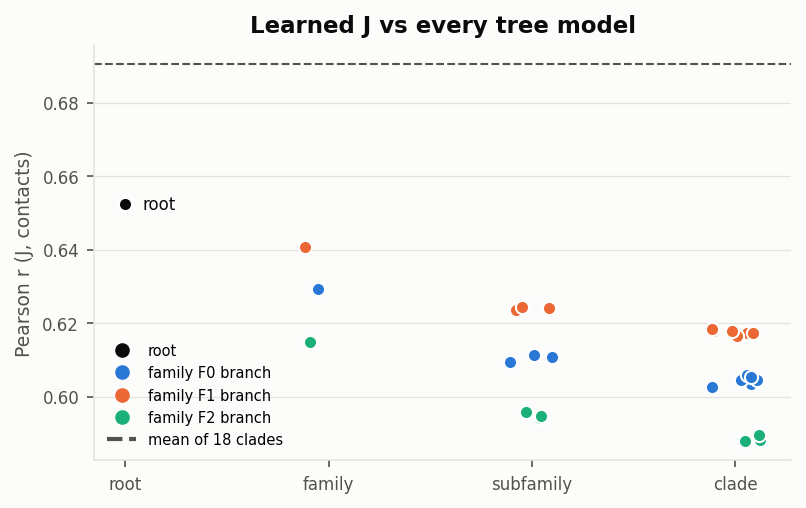
\includegraphics[width=0.49\linewidth]{models/fa_unconditional_H128/tree_rJ.png}\hfill
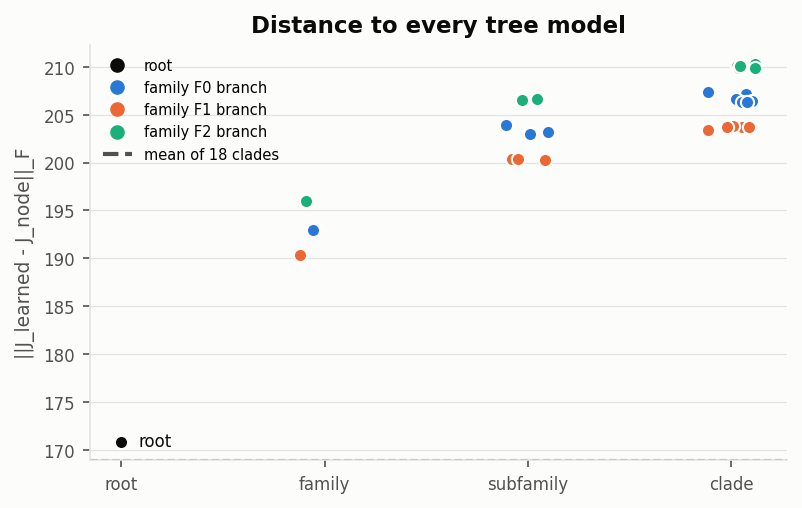
\includegraphics[width=0.49\linewidth]{models/fa_unconditional_H128/tree_dJ.png}
\caption{Learned $J$ vs every model of the tree, grouped by level, coloured by family branch. Left: Pearson
correlation on the contact entries. Right: distance $\|J^0_{\text{learned}}-J^0_{\text{node}}\|_F$. Dashed:
the average of the 18 clade models.}
\label{fig:treeJ}
\end{figure}

\begin{center}\small
\begin{tabular}{lccccc}
\toprule
compared with & $r_J$ (contacts) & slope & $d_J$ & $r_h$ & $d_h$\\
\midrule
average of the 18 clades & \textbf{0.691} & 0.57 & \textbf{168.9} & \textbf{0.922} & \textbf{26.3}\\
root (ancestor) & 0.652 & 0.57 & 170.9 & 0.865 & 27.5\\
family F0 & 0.629 & 0.48 & 192.9 & 0.836 & 36.2\\
family F1 & 0.641 & 0.49 & 190.3 & 0.857 & 35.3\\
family F2 & 0.615 & 0.47 & 196.0 & 0.802 & 39.3\\
subfamilies (range) & 0.594--0.624 & 0.43--0.46 & 200--207 & 0.78--0.84 & 38--42\\
clades (range) & 0.588--0.618 & 0.42--0.45 & 203--210 & 0.77--0.83 & 39--44\\
\bottomrule
\end{tabular}
\end{center}

\begin{figure}[H]
\centering
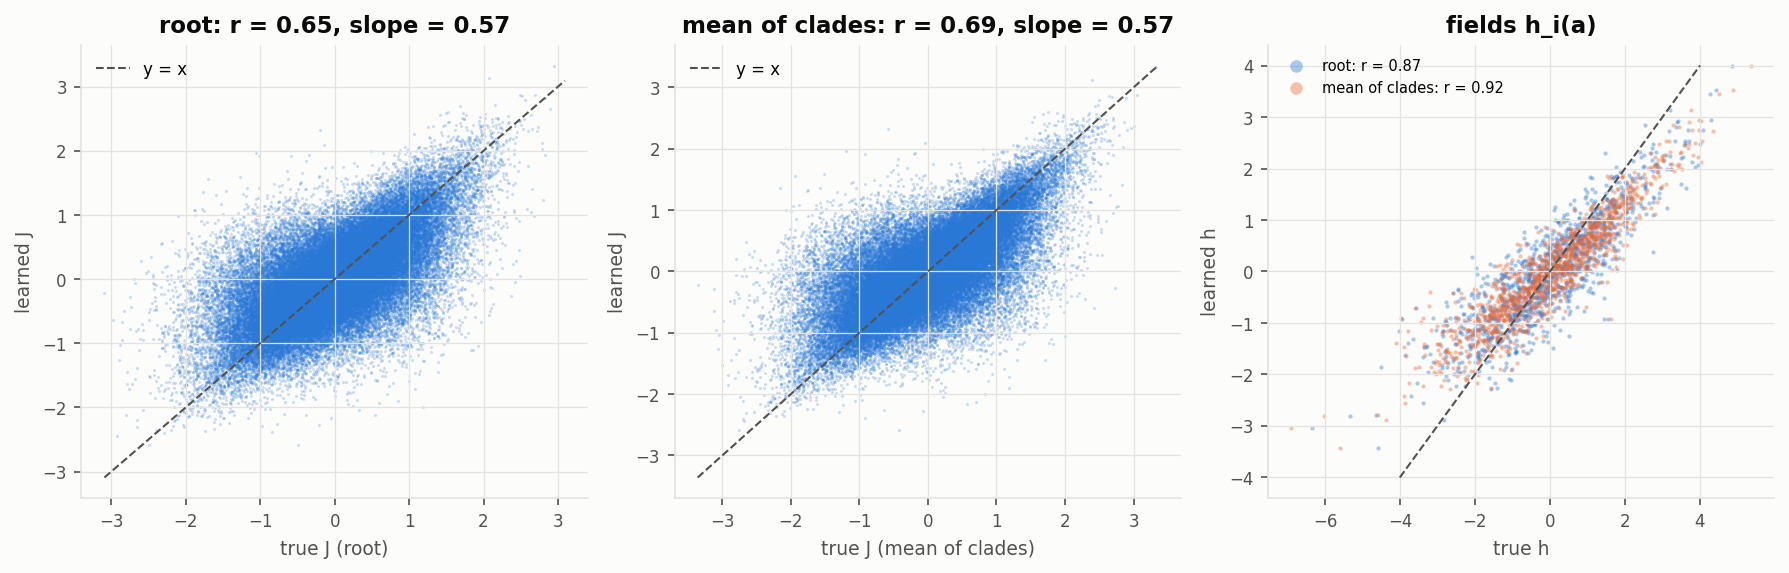
\includegraphics[width=\linewidth]{models/fa_unconditional_H128/tree_scatter_J.png}
\caption{Learned vs true couplings on the contact entries, for the root and for the average of the clades,
and learned vs true fields. The cloud is centred on a line of slope $\approx0.57$, below the diagonal.}
\end{figure}

\paragraph{Reading.}
\begin{enumerate}
\item \textbf{The model learned the common ancestor, not any family.} The similarity decreases
monotonically down the tree: root/average of clades $>$ families $>$ subfamilies $>$ clades
(Figure~\ref{fig:treeJ}). This is what one expects from fitting one Potts model to all 18 clades: the part of
$J$ shared by everyone is the ancestral part, and the family- and clade-specific perturbations average out.
The best match is the average of the clades ($r_J=0.69$), which is itself close to the root (distance 71,
against $\|J_{\text{root}}\|=202$).
\item \textbf{F2 is the \emph{least} similar family}, although it is the most over-generated. The wrong
family weights are therefore not caused by $J$ resembling F2. They sit in the global balance of $h$ and
$J$ that PL does not constrain.
\item \textbf{The couplings are too weak and partly misplaced.} The slope is 0.57: along the direction of
the true couplings, the learned ones have about 57\% of the true magnitude. This is the source of the
too-weak correlations. The distance to the root, 171, splits into 160 on the true contacts and 61 on
non-contacts, where the truth is zero but the learned model has spread couplings (mean $|J|=0.06$). The
learned contact couplings have almost the right total size (177 vs 202), but only part of them is aligned
with the true ones. The rest encodes the mixture: extra couplings that tie together the residues typical of
each family. That is exactly how a single Potts model can mimic a mixture.
\item \textbf{The contact map is found perfectly.} All 120 true long-range contacts are the 120 top-ranked
pairs by $\|J_{ij}\|$ with APC (precision $1.00$). This holds even with $H=128<179$ heads. The heads are
enough to locate every contact, though not to reproduce every coupling value.
\item The fields agree well with the average of the clades ($r_h=0.92$): conservation is learned correctly.
\end{enumerate}

\subsection{Summary of the first run}
\begin{keybox}{Unconditioned model with $H=128$}
\begin{itemize}[nosep]
\item[+] Finds all true contacts; site frequencies inside each family are right; no copies of test
      sequences; pooled correlations $r_C=0.90$ (0.95 once family shares are corrected).
\item[--] \textbf{Wrong family weights} (22/12/66\% instead of 33/33/33\%). This is a property of the
      learned distribution, not of the sampler, and is explained by pseudo-likelihood not seeing $Z$.
\item[--] Correlations about 20--35\% too weak (slope 0.63--0.79), because the couplings are shrunk
      (slope 0.57) and partly spent on representing the mixture.
\item[$\to$] Its $J$ is closest to the \emph{ancestral} (root) and \emph{average} models, and gets steadily
      further from the family, subfamily and clade models. It learned what all clades share.
\end{itemize}
Natural next steps: the conditioned model (tags fix the family weights and allow clade-specific $J$);
$H=256$ and/or more epochs to see how much of the shrinkage is capacity vs the mixture.
\end{keybox}
